\documentclass{article}
\usepackage{amsmath}
\usepackage{amssymb}
\usepackage{tikz}
\usetikzlibrary{automata,positioning}

\begin{document}

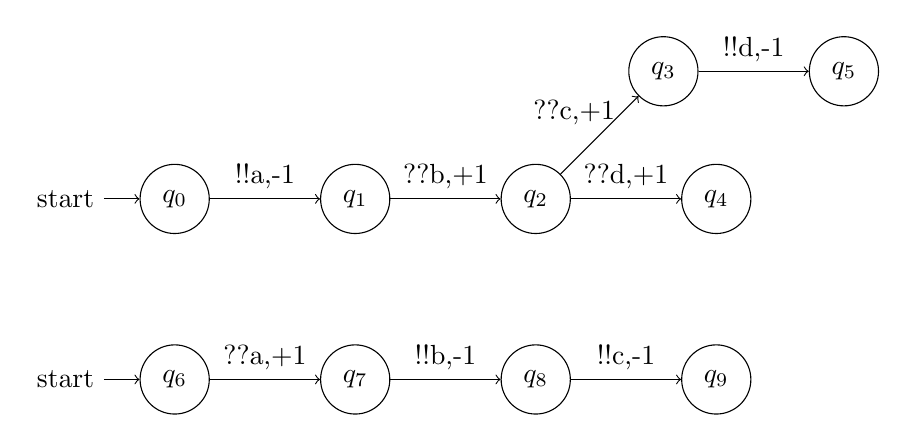
\begin{tikzpicture}[->,node distance = 1.4cm]
		\node[state,initial] (q_0) {$q_0$};
		\node[state] (q_1) [right = of q_0] {$q_1$};
		\node[state] (q_2) [right = of q_1] {$q_2$};
		\node[state] (q_3) [above right = of q_2] {$q_3$}; 
		\node[state] (q_4) [right = of q_2] {$q_4$};
		\node[state] (q_5) [right = of q_3] {$q_5$};
		\node[state,initial] (q_6) [below = of q_0] {$q_6$};
		\node[state] (q_7) [right = of q_6] {$q_7$};
		\node[state] (q_8) [right = of q_7] {$q_8$};
		\node[state] (q_9) [right = of q_8] {$q_9$};
		
		\draw (q_0) edge[above] node{!!a,-1} (q_1);
		\draw (q_1) edge[above] node{??b,+1} (q_2);
		\draw (q_2) edge[above] node{??c,+1 $\hspace{15pt}$} (q_3);
		\draw (q_2) edge[above] node{??d,+1} (q_4);
		\draw (q_3) edge[above] node{!!d,-1} (q_5);
		\draw (q_6) edge[above] node{??a,+1} (q_7);
		\draw (q_7) edge[above] node{!!b,-1} (q_8);
		\draw (q_8) edge[above] node{!!c,-1} (q_9);
		\end{tikzpicture}

\end{document}